\documentclass[a4paper,12pt]{article} 
\usepackage[utf8]{inputenc} 
\usepackage[italian]{babel} 
\usepackage{enumerate}
\usepackage{enumitem}
\usepackage{graphicx}
\usepackage{listings}
\usepackage{wrapfig}
\usepackage[a4paper,top=3cm,bottom=3cm,left=3cm,right=3cm]{geometry}
\usepackage{array}
\usepackage{hyperref}
\usepackage{float}
\setlength\extrarowheight{2pt}

\usepackage[Algoritmo]{algorithm}
\usepackage{algpseudocode}

\usepackage{graphicx}
\usepackage{subcaption}

\title{\bf Classificazione di cellule epiteliali HEp-2 mediante l'utilizzo dei tensori di Fisher} 
\date {27 Agosto 2015}
\author{Lorenzo Cioni\\\textit{{\small lore.cioni@gmail.com}}}

\begin{document}
\maketitle

\begin{abstract}

Analizzare e classificare le cellule epiteliali di tipo 2 (HEp-2) mediante l'utilizzo della tecnica della immunofluorescenza indiretta è uno standard per rilevare malattie al tessuto connettivo umano, come ad esempio l'Artrite Reumatoide. Purtroppo questo metodo è molto costoso in termini di tempo e di lavoro impiegato e particolarmente soggettivo.

Questo elaborato ha come finalità quella di implementare un metodo per la classificazione di questo tipo di cellule basato sull'utilizzo del descrittore di covarianza e dei tensori di Fisher per l'estrazione di \emph{features} dalle immagini.
\end{abstract}

\tableofcontents

\section{Introduzione}

Una delle procedure standard per il rilevamento di malattie al tessuto connettivo umano, come ad esempio l'Artrite Reumatoide o il Lupus, è l'utilizzo di Immunofluorescenza Indiretta sulle cellule epiteliali di tipo 2, altrimenti conosciute come HEp-2.

Questo tipo di analisi ha due principali svantaggi: è molto soggettiva e richiede un gran numero di ore lavorative. Si è così pensato ad un metodo per automatizzare il processo per ottenere risultati migliori sia sotto il profilo medico che dal punto di vista di tempo impiegato.

Il metodo proposto e implementato è tratto da un articolo pubblicato in occasione del contest di \emph{Pattern Recognition 2014 \footnote{ICPR Contest 2014 - http://nerone.diem.unisa.it/hep2contest/description.shtml}} [1]. Per la classificazione delle cellule si procede inizialmente all'estrazione di un adeguato numero di \emph{features} attraverso l'utilizzo del \emph{Descrittore di Covarianza} [2], vengono poi utilizzati i \emph{Tensori di Fisher} che codificano informazioni addizionali rispetto alla distribuzione delle \emph{features} ed infine le cellule vengono classificate tramite un SVM multiclasse.

I test per la valutazione della bontà del metodo sono stati effettuati sul dataset della competizione\footnote{HEp-2 Dataset - http://mivia.unisa.it/datasets/biomedical-image-datasets/hep2-image-dataset/}.

\section{Tecniche utilizzate}

Vengono ora presentate le tecniche utilizzate all'interno del programma: l'estrazione di \emph{features} dall'immagine mediante l'utilizzo dei \emph{filtri di Gabor}, il Descrittore di Covarianza (\emph{Covariance Descriptor}), il Modello Mistura di Gaussiane (\emph{Gaussian Mixture Model, GMM}) e i Tensori di Fisher (\emph{Fisher Tensors}).

\subsection{Il filtro di Gabor}

I filtri di Gabor\footnote{Gabor, D.: \emph{Theory of communication.} In J. IEE, vol. 93, pp. 429-457, Londra, 1946.} sono filtri passa-banda usati nell'analisi di immagini principalmente per l'estrazione di \emph{features} e l'analisi basata sulla tessitura.

La risposta finita all'impulso di questi filtri è calcolata come prodotto di uno sviluppo Gaussiano con oscillazione complessa. Estendendo queste funzioni a due dimensioni è possibile creare filtri sensibili all'orientazione\footnote{Daugman, J. G.: \emph{Uncertainty relation for resolution in space, spatial frequency, and orientation optimized by two-dimensional visual cortical filters} J. Optical Society of America A, vol. 2, no. 7, pp. 1160-1169, July 1985.} e sotto certe condizioni è possibile approssimare linearmente la fase.

Sia $(x, y)$ un punto dell'immagine. L'equazione per il filtro di Gabor 2D è la seguente:

$$G(x, y) = e^{(- \frac{(x')^2 + \gamma^2 (y')^2}{2 \sigma^2})} \cos (2 \pi \frac{x'}{\lambda})  $$ 

con 

$$x' = x \cos \theta + y \sin \theta$$
$$y' = - x \cos \theta + y \sin \theta$$

I parametri del filtro sono:
\begin{itemize}
\item $\theta$: orientazione del filtro, espressa in gradi.
\item $\lambda$: lunghezza d'onda del fattore coseno, espressa in pixels.
\item $\gamma$: specifica l'ellitticità del supporto della funzione di Gabor.
\item $\sigma$: è il parametro che regola l'inviluppo Gaussiano.
\end{itemize}

\begin{figure}[H] 
  \centering
    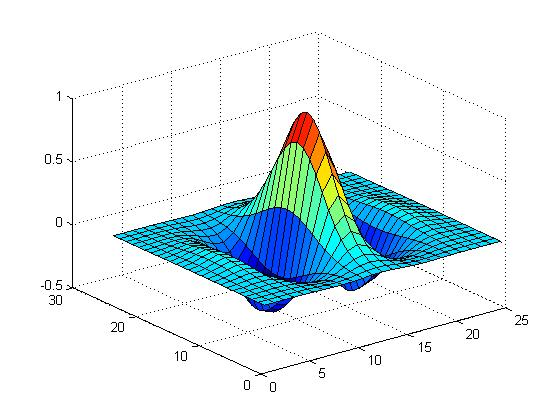
\includegraphics[width=0.5\textwidth]{images/gaborfilter.jpg}
    \vspace{-0.5cm}
    \caption{{\small \textit{Esempio di filtro di Gabor 2D}}}
\end{figure}

Al fine di estrarre utili \emph{features} da un'immagine è utile utilizzare un set di filtri di Gabor con parametri diversi, ad esempio la scala e l'orientazione.

Nel programma viene utilizzato un set di filtri di Gabor con 4 diverse angolazioni e 3 diverse scale per un totale di 12 filtri:

\begin{figure}[H] 
  \centering
    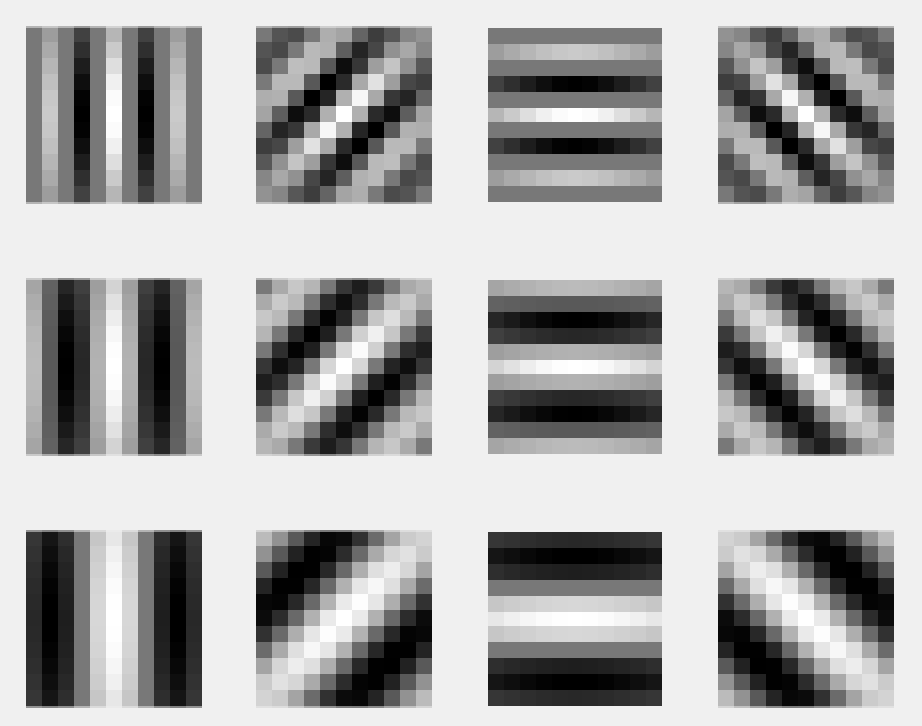
\includegraphics[width=0.5\textwidth]{images/filterbank.png}
    \caption{{\small \textit{Set di filtri di Gabor con 4 angolazioni e 3 scale}}}
\end{figure}

Per ciascun pixel dell'immagine viene dunque calcolato il vettore delle \emph{features} ottenute mediante la convoluzione dell'immagine con i filtri di Gabor (dividendo la parte reale dalla parte immaginaria).

\subsection{Descrittore di Covarianza}

Il Descrittore di Covarianza (Covariance Descriptor\footnote{Oncel Tuzel, Fatih Porikli, Peter Meer, \emph{Region Covariance: A Fast Descriptor for
Detection and Classification} Mitsubishi Electric Research Laboratories, Inc., 2006.}, CovD) viene utilizzato in letteratura per descrivere e caratterizzare regioni di immagini. 

Data un'immagine con associato, a ciascun pixel, un vettore di \emph{features}, il Descrittore di Covarianza codifica informazioni che riguardano le \emph{varianze} di queste ultime all'interno di una regione, la loro correlazione e la loro distribuzione nello spazio. Questo metodo è molto utilizzato in particolare modo quando si ha bisogno di rimanere invarianti rispetto all'illuminazione o alla rotazione.

Data un'immagine $I$ con associato, per ciascun pixel $(x, y)$, il vettore di features di dimensione $d$, si considera $F$ come l'immagine di features a $d$ livelli. Viene dunque considerata una regione di F tale che $R \subset F$ e consideriamo $\{f_i\}_{i = 1,\ldots, n} \in R$ la $i$-esima features, con $n$ numero di pixels della regione.

A questo punto la regione $R$ viene rappresentata da una matrice di covarianza di dimensione $d X d$ dei \emph{features points}:

$$C = \frac{1}{n -1} \sum_{k = 1}^{n} (f_k - \mu)(f_k - \mu)^T$$

con $\mu$ la media dei \emph{features points}.

Poichè la matrice $C$ è definita positiva e simmetrica può essere considerata un \emph{tensore}.



\section{Algoritmo}

Utilizzando le tecniche descritte nella sezione precedente è stato ideato l'algoritmo descritto in [1].

L'algoritmo può essere suddiviso in 4 parti fondamentali:
\begin{enumerate}
\item Creazione dei filtri di Gabor
\item Estrazione di features
\item Creazione di un modello a mistura di gaussiane
\item Calcolo dei \emph{tensori di fisher}
\item Classificazione
\end{enumerate}

Inizialmente viene creato il set di filtri di Gabor, impostando 4 diverse orientazioni e 3 diverse scale. Si ottengono così 12 filtri distinti che verranno utilizzati nella fase di estrazione delle \emph{features}.

\subsection{Estrazione delle \emph{features}}

In questa fase ciascuna scansione viene elaborata al fine di estrarre delle \emph{features}. 

Inizialmente, data un immagine viene calcolata la sua maschera, ovvero un'immagine binaria che evidenzia i pixels di \emph{foreground}. In questo modo il calcolo delle \emph{features} verrà effettuato solamente sui pixels rilevanti dell'immagine, escludendo lo sfondo. La maschera viene calcolata mediante un'operazione di sogliatura tramite il metodo di Otsu.

L'immagine viene scansionata a blocchi quadrati di dimensione 80 pixels, sovrapposti con un passo di 20 pixels.

\begin{figure}[H]
\captionsetup[subfigure]{labelformat=empty}
\begin{subfigure}{.5\textwidth}
\centering
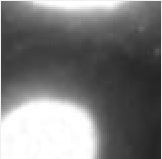
\includegraphics[height=1.6cm]{images/block.png}
\caption{Blocco}
\end{subfigure}%
\begin{subfigure}{.5\textwidth}
\centering

\includegraphics[height=1.8cm]{images/mask.png}
\caption{Maschera}
\end{subfigure}%
\caption{Esempio di blocco e maschera di elaborazione}
\end{figure}

A questo punto, considerando solo i pixel del blocco filtrati dalla maschera, per ciascun pixel viene estratto un vettore di 15 osservazioni così composto:

$$F_{x,y} = [I(x, y), x, y, |G_{0,0}(x, y)|, \ldots, |G_{0, v}(x, y)|, |G_{1, 0}(x, y)|, \ldots, |G_{u, v}(x, y)|]$$

dove 
\begin{itemize}
\item $I(x, y)$ è il livello di grigio del pixel alla posizione $(x, y)$.
\item $x, y$ solo rispettivamente l'ascissa e l'ordinata del pixel considerato.
\item $u$ è il numero delle scale del filtro di Gabor (in questo caso 3).
\item $v$ è il numero delle orientazioni del filtro di Gabor (in questo caso 4).
\end{itemize}

A questo punto a ciascun pixel del blocco è associato un vettore di 15 osservazioni, dunque la matrice delle \emph{features} avrà dimensione $15\; X\; n^2$, con $n$ dimensione del blocco (in questo caso 80).
Si procede dunque con il calcolo del \emph{descrittore di covarianza} del blocco, ottenendo una matrice $C$ di dimensione $15 \; X \; 15$.

Gli elementi della diagonale di questa matrice rappresentano le varianze di ciascuna osservazione e gli elementi extra diagonali rappresentano le correlazioni. 

In ultima istanza viene effettuato il \emph{mapping} sullo spazio tangente per ricondurci alla geometria Riemanniana.

\begin{figure}[H] 
  \centering
    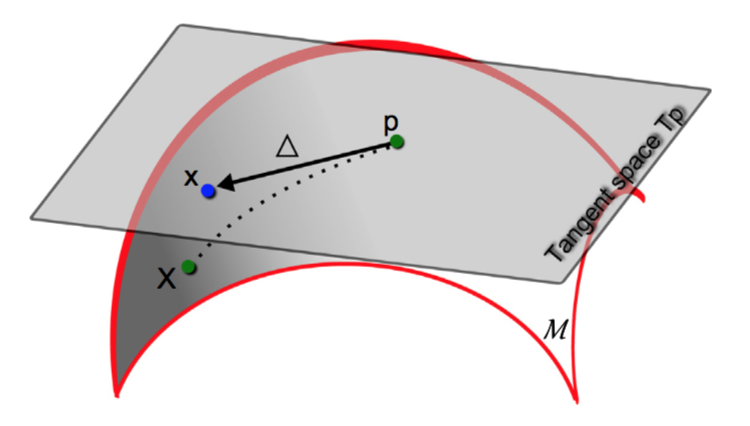
\includegraphics[width=0.5\textwidth]{images/tangent_space.png}
    \caption{{\textit{Illustrazione dello spazio tangente $T_P$ al punto $P$ sulla varietà Riemanniana $\mathcal{M}$}}}
\end{figure}

Il vettore tangente $\Delta$ può essere ottenuto mediante mappa logaritmica, $\Delta = \log(C)$.

\subsection{Creazione di un modello a mistura di gaussiane}

A partire dalle \emph{features} estratte in precedenza si procede ora alla creazione di un modello a mistura di gaussiane. Viene fissato un valore di $K$, nel nostro caso 16, un valore di \emph{tolleranza} e un un numero massimo di \emph{iterazioni}.

Il modello così creato verrà utilizzato per il calcolo dei tensori di Fisher.

\subsection{Calcolo dei \emph{tensori di Fisher}}

Per ciascuna immagine vengono ora calcolati i \emph{tensori di Fisher}. Dati in ingresso:
\begin{itemize}
\item $\mathbf{Q} = \{ Q_t \}_{t = 1}^{p}$ descrittori di covarianza estratti da una immagine ($p$ numero di blocchi).
\item $\lambda_i = \{\omega_i, \mu_i, \Sigma_i\}$, componenti della mistura di gaussiane, con $i = 1, \ldots, K$
\end{itemize}

Sia $p(x| \lambda)$ una distribuzione di probabilità modellata da una GMM con K gaussiane

$$p(x | \lambda) = \sum_{i = 1}^{K} \omega_i g(x | \mu_i, \mathcal{\sum}_i)$$

\begin{algorithm}[H]
\caption{Tensore di Fisher di $\mathbf{Q}$}
\begin{algorithmic}
\State - Calcolo della rappresentazione logaritmica euclidea di $\mathbf{Q}$, $q_t = Vec(\log(\mathbf{Q}))$
\State - $\gamma_i(q_t) = \frac{\omega_i g(q_t | \mu_i, \sum_i)}{\sum_{j=1}^{K} \omega_j g(q_t | \mu_j , \sum_j)}$
\For {$i = 1, \ldots, K$}
\State $\mathcal{G}_i = \frac{1}{p\sqrt{\omega_i}} \sum_{t = 1}^{p} \gamma_i(q_t) \sigma_{i}^{-1} (q_t - \mu_i) $ con $\sum_i = \sigma_{i}^{2}$
\EndFor
\State - $FT(\mathbf{Q}) = [\mathcal{G}_{1}^T, \ldots, \mathcal{G}_{K}^T]$
\end{algorithmic}
\end{algorithm}

\subsection{Classificazione}

Infine si procede con la classificazione, affidata al classificatore SVM. 

Viene creato il modello multiclasse con cross-validazione basato su kernel gaussiano, suddividendo il dataset in 8 parti uguali. 

Il modello viene poi valutato andando a predire l'intero dataset.
\section{Dataset}

Per la valutazione dell'efficienza dell'algoritmo implementato è stato utilizzato una parte del dataset dell'\emph{ICPR HEp-2 Cell Classification Contest}.

Il dataset contiene al suo interno 149 immagini che rappresentano le scansioni di vetrini di laboratorio. All'interno di queste immagini è possibile distinguere 9 diversi pattern: \emph{punteggiato}, \emph{nucleolare}, \emph{citoplasmico}, \emph{omogeneo}, \emph{granulare}, \emph{negativo} e \emph{centromero}. Alcune immagini del dataset sono poi classificate come \emph{altro}, rendendo difficile una loro classificazione, questi elementi sono stati dunque non considerati. A causa del basso numero di elementi classificati con \emph{centromero} anche questi sono stati rimossi fino ad ottenere un totale di 137 immagini.

Le immagini sono state acquisite tramite un microscopio a fluorescenza (40 ingrandimenti) in combinazione con una lampada di mercurio vaporizzato a 50W e una fotocamera digitale SLIM con risoluzione 1920 x 1110.

\begin{figure}[H] 
  \centering
    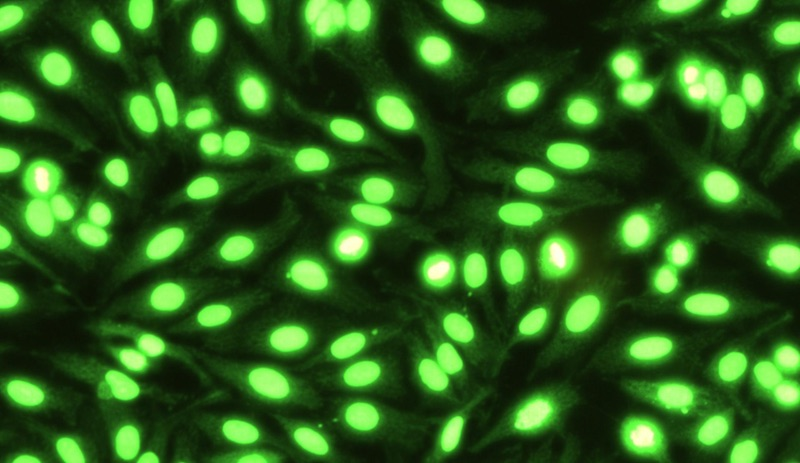
\includegraphics[width=0.9\textwidth]{images/example.jpg}
    \caption{{\small \textit{Esempio di immagine del dataset}}}
\end{figure}

Ciascuna immagine è stata poi annotata da un medico specialista ed associata ad una delle classi di pattern sopra esposte. Le annotazioni sono state inserite in una tabella così da poterne ricavare un \emph{training set}.

\begin{figure}[H]
\captionsetup[subfigure]{labelformat=empty}
\begin{subfigure}{.16\textwidth}
\centering
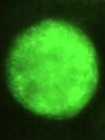
\includegraphics[height=1.6cm]{images/omogeneo.jpg}
\caption{Omogeneo}
\end{subfigure}%
\begin{subfigure}{.16\textwidth}
\centering
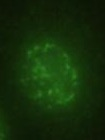
\includegraphics[height=1.8cm]{images/nucleolare.jpg}
\caption{Nucleolare}
\end{subfigure}%
\begin{subfigure}{.16\textwidth}
\centering
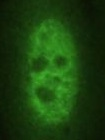
\includegraphics[height=1.8cm]{images/punteggiato.jpg}
\caption{Punteggiato}
\end{subfigure}%
\begin{subfigure}{.16\textwidth}
\centering
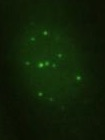
\includegraphics[height=1.8cm]{images/granulare.jpg}
\caption{Granulare}
\end{subfigure}%
\begin{subfigure}{.16\textwidth}
\centering
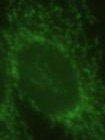
\includegraphics[height=1.8cm]{images/citoplasmico.jpg}
\caption{Citoplasmico}
\end{subfigure}%
\begin{subfigure}{.16\textwidth}
\centering

\includegraphics[height=1.8cm]{images/negativo.jpg}
\caption{Negativo}
\end{subfigure}%
\caption{Esempi di cellule classificate nel dataset}
\end{figure}

\section{Risultati}
\section{Implementazione}

L'implementazione dell'algoritmo qui presentato è stata sviluppata interamente in codice Matlab, compatibile con la versione 2014a o successive. 
Per una corretta esecuzione è necessario avere installato alcuni pacchetti aggiuntivi:

\begin{itemize}
\item \emph{Image Acquisition Toolbox}: nesessario per l'elaborazione di immagini.
\item \emph{Image Processing Toolbox}: necessario per l'elaborazione di immagini.
\item \emph{Statistics and Machine Learning Toolbox}: necessario per la creazione del modello per la classificazione SVM e per la creazione di un modello a mistura di gaussiane.
\end{itemize}

Per la creazione del \emph{train set} di partenza viene utilizzata una funzione Matlab per il \emph{parsing} di valori da file in formato virgola mobile. In caso di diverse necessità sarà sufficiente modificare questa funzione senza interferire con il resto dell'esecuzione.

\subsection{Configurazioni iniziali}

Le configurazioni sono tutte racchiuse all'interno di un'unica classe, così da poter essere facilmente adattabile all'esecuzione su macchine diverse. 

Il file \textbf{configuration.m} contiene al suo interno le configurazioni di base del progetto: è necessario modificarle prima di proseguire con l'esecuzione del programma.

\begin{itemize}
\item \textbf{image\_path}: cartella dove si trovano le immagini da analizzare.
\item \textbf{image\_prefix}: prefisso del nome dei file.
\item \textbf{image\_ext}: estensione dei file.
\item \textbf{validation\_file}: file in formato CSV per la creazione del \emph{training set}.
\item \textbf{resize}: \emph{true/false}, se vero le immagini verranno ridimensionate. Permette un'esecuzione più rapida del programma, ma viene meno l'accuratezza finale.
\item \textbf{resizeTo}: imposta la dimensione alla quale ridimensionare l'immagine (se impostato il \emph{resize} a \emph{true}).
\item \textbf{K}: numero di gaussiane per la creazione del modello a mistura.
\end{itemize}

\subsection{Esecuzione}

L'algoritmo, come descritto nella Sezione 3 è stato suddiviso in 5 fasi fondamentali, da eseguire in ordine.

\begin{enumerate}
\item \textbf{loadTrainingSet.m}: si occupa della creazione del \emph{training set}. Legge il file CSV e va a creare una struttura contenente:
\begin{itemize}
\item ID dell'immagine.
\item \emph{Label} assegnata.
\item Nome completo del file e cartella.
\end{itemize}
\item \textbf{extractImages.m}: esegue quanto descritto nella Sezione 3.1. 
\item \textbf{runGMM.m}: esegue quanto descritto nella Sezione 3.2.
\item \textbf{saveSignatures.m}: calcola i tensori di Fisher nel modo descritto nella Sezione 3.3.
\item \textbf{runSVM.m}: esegue la classificazione. Viene stampata la tabella dei risultati ottenuti e mostrata una versione grafica della matrice di confusione (generata tramite la funzione \textbf{plotConfusionMatrix.m}).
\end{enumerate}

\section{Conclusioni}

La tecnica utilizzata per la classificazione di cellule epiteliali HEp-2 ha dato risultati positivi sul dataset considerato.

Buona parte, circa il 70\%, delle scansioni sono state correttamente classificate, in particolare la tecnica è molto buona per scartare i campioni negativi, riconosciuti con un'alta accuratezza.

Alcuni dei pattern sono però difficilmente classificabili: questo a causa anche del basso numero di campioni di training a disposizione che non consentono così la creazione di un modello adeguato.

Un possibile miglioramento potrebbe essere ottenibile aumentando il numero di filtri di Gabor utilizzati, andando a estrarre un numero maggiore di osservazioni dall'immagine e rendendo più accurata la descrizione delle singole classi, andando però ad aumentare la durata di computazione.

In conclusione il metodo presentato in [1] e qui implementato è una buona soluzione al problema di classificazione di cellule, migliorabile nella fase di estrazione delle \emph{features} e nella scelta dei parametri.

\begin{thebibliography}{1}

\bibitem{}
Masoud Faraki, Mehrtash T. Harandi, Arnold Wiliem, Brian C. Lovell, \emph{Fisher tensors for classifying human epithelial cells}.\hskip 1em plus
  0.5em minus 0.4em\relax Pattern Recognition, Volume 47, 2014, pp. 2348 - 2359.

\bibitem{}
Oncel Tuzel, Fatih Porikli, Peter Meer, \emph{Region Covariance: A Fast Descriptor for
Detection and Classification}.\hskip 1em plus
  0.5em minus 0.4em\relax Mitsubishi Electric Research Laboratories, Inc., 2006.

\bibitem{}
Gabor, D.: \emph{Theory of communication} In J. IEE, vol. 93, pp. 429-457, London, 1946.

\end{thebibliography}



\end{document}